%==============================================================================
% @author Clinton Freeman <freeman@cs.unc.edu>
% @date 2014-11-26
%==============================================================================

\FloatBarrier
\section{Case Study: Randomized Incremental Delaunay Triangulation}
\label{sec:case-delaunay}

In this section, we use the workbench to implement and visualize a randomized
incremental Delaunay triangulation algorithm~\cite{lischinski1994incremental}.
We use the algorithm to construct \emph{polyhedral terrains}, or graphs of
continuous functions that are piecewise linear. The algorithm takes as input a
special point set called a terrain. A \emph{terrain} is a 2-dimensional surface
in 3-dimensional space with a special property: every vertical line intersects
it in a point, if it intersects it at all. The algorithm produces as output a
triangulation that is \emph{Delaunay}: the circumcircle of any triangle in the
triangulation does not contain any input points in its interior. 

\begin{figure}[htb]
\centering
\shadowimage[width=\textwidth]{figures/delaunay-terrain-intro} 
\caption{A polyhedral terrain produced by the workbench.}
\label{fig:terrain-intro} 
\end{figure}

Our workbench already has a simple point set type
(\texttt{PointSet\_3r}), but we will need to introduce a new type 
(\texttt{Terrain\_3r}) and visualize its methods in order to animate the
algorithm. The algorithm uses the quad-edge data
structure~\cite{guibas1985primitives} to store and manipulate terrain topology.
After explaining how the algorithm and data structure work, we use Heckbert's
QuadEdge C++ library to implement \texttt{Terrain\_3r} and use it to arrive at a
correct implementation of incremental Delaunay. We conclude by using the GUI to
generate an input point set and run the algorithm.

%==============================================================================

\subsection{Algorithm Overview}

The algorithm starts with an initial triangle, constructed such that it contains
all input points and is large enough to not affect the points' triangulation.
Points are inserted one at a time in a random order. Each insertion maintains
the invariant that the triangulation is Delaunay. There are three steps to
inserting a point $p$: localizing $p$ to a triangle $T$, inserting $p$ into
$T$, and restoring the Delaunay invariant. The insertion is a constant time
operation that adds three new edges from the triangles vertices to $p$. Below,
we describe localizing $p$ and restoring the invariant.

We start by finding the triangle that contains $p$. We could achieve optimal
$O(\log n)$ time, but this requires maintaining a complicated data structure.
Instead, we use the naive strategy of iterating over all triangles,
performing containment tests.  This strategy is incredibly easy to implement and 
- if the points are randomly chosen from a uniform distribution - only requires
$O(n^{1/2})$ operations in expectation. Once we locate $T$, we insert $p$ and
move to restore the Delaunay invariant.

We restore the invariant through a series of edge flips. Let $T = abc$ be the
old Delaunay triangle containing $p$, with circumcircle $C$. Then the new edges
$\seg{pa}$, $\seg{pb}$, and $\seg{pc}$ are Delaunay: the circle passing through
$p$ and tangent to $C$ at $a$ is a site-free witness for the Delaunayhood of the
edge $\seg{pa}$ (we can argue analogously for $\seg{pb}$ and $\seg{pc}$). The
edges $\seg{ab}$, $\seg{ac}$, $\seg{bc}$ are {\em suspect} since we do not know
if they pass the \textsc{InCircle} test with respect to $p$ and the triangle on
their other side. We have to check these suspect edges; if an edge fails the
\textsc{InCircle} test then it will be swapped, creating a new Delaunay edge
emanating from $p$ and creating two new suspect edges that must now be tested.
This process continues recursively until the invariant is restored.

%==============================================================================

\FloatBarrier
\subsection{The Quad-edge Data Structure}

The algorithm operates on the quad-edge data structure, which can be used to
represent planar subdivisions or manifold polytopes in 3D. The quad-edge is an
easy to use alternative to the earlier winged-edge data structure by
Baumgart~\cite{baumgart1975polyhedron} that has the added benefit of
simulaneously representing a graph and its dual.
Guibas and Stolfi describe the quad-edge structure in great
detail~\cite{guibas1985primitives}; for our purposes we can just familiarize
ourselves with the high level API provided by Heckbert's C++ quad-edge library.

In the quad-edge data structure, there are classes for vertices, edges, and
faces, but edges play the leading role. The edges store complete topological
information; all of the topological information stored by the faces and vertices
is redundant with information in the edges. The \texttt{Edge} class represents a
directed edge. Given \texttt{Edge *e}, you can find the immediately adjacent
vertices, faces, and edges, and the ``symmetric'' edge that points in the
opposite direction. These operators are all fast (just a few memory references).
Because edges are oriented, we can speak of the origin and destination vertices
and left and right faces of an edge. Figure \ref{fig:quadedge-edge-api}
summarizes the \texttt{Edge} API.

\begin{figure}[h]
	\centering
	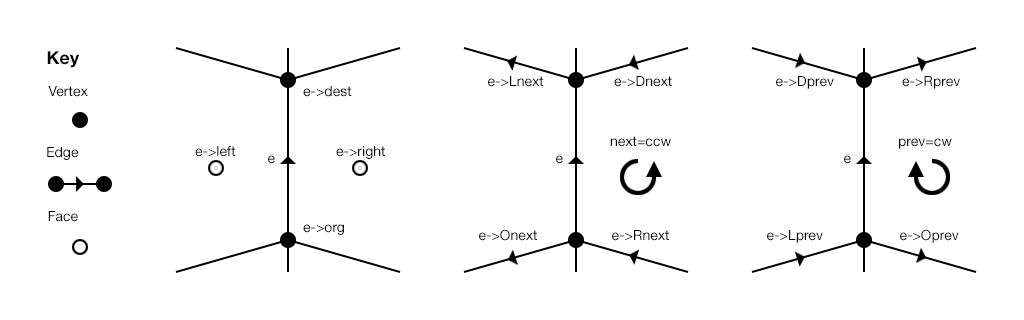
\includegraphics[width=\textwidth]{figures/quadedge-edge-api} 
	\caption{Pictoral summary of the \texttt{Edge} API.}
	\label{fig:quadedge-edge-api} 
\end{figure}

The \texttt{Vertex} and \texttt{Face} classes are simple. The information stored
at a vertex consists of one piece of topological information (a pointer to one
of the outgoing edges of the vertex), plus geometric information (the (x, y, z)
position), and optional attribute information (color, normals, etc). Each face
stores one piece of topological information, a pointer to one of the
ccw-oriented edges of the face, plus optional attribute information (color, etc).

The \texttt{Cell} class models a single subdivision, which includes sets of
vertices, edges, and faces. The routines you will need most are those depicted
in figure \ref{fig:quadedge-cell-api}. These are called Euler operators, since
they maintain Euler's formula $V-E+F=2$ interrelating the number of vertices,
edges, and faces of a planar graph. If the topology is a valid graph before the
call, it will be valid after the call, as well.

\begin{figure}[h]
	\centering
	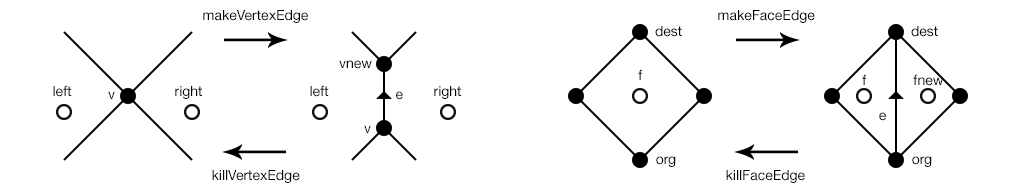
\includegraphics[width=\textwidth]{figures/quadedge-cell-api} 
	\caption{Pictoral summary of the 4 major \texttt{Cell} operations.}
	\label{fig:quadedge-cell-api} 
\end{figure}

\begin{itemize}
  \item \texttt{c->makeVertexEdge(v, left, right)} splits vertex \texttt{v},
  creating a new edge and vertex that both lie between faces \texttt{left} and
  \texttt{right}. The new edge has \texttt{left} on its left and \texttt{right}
  on its right, \texttt{v} at its origin and the new vertex at its destination.
  The new edge is returned; the new vertex is easily found by taking
  \texttt{Dest()} of the return value. The new vertex and edge are stored in the
  sets associated with cell \texttt{c}. If \texttt{left} and \texttt{right} are
  not adjacent to \texttt{v} then an error message will be printed and core
  dumped.
  \item \texttt{c->makeFaceEdge(f, org, dest)} is the dual of this. It splits
  face \texttt{f}, creating a new edge and face that both lie between vertices
  \texttt{org} and \texttt{dest}. The new edge has \texttt{org} as its origin
  and \texttt{dest} as its destination, \texttt{f} as its left face and the new
  face as its right face. The new edge is returned; the new face is easily found
  by taking \texttt{Right()} of the return value. The new face and edge are
  stored in the sets associated with cell \texttt{c}. If \texttt{org} and
  \texttt{dest} are not adjacent to \texttt{f} then an error message will be
  printed and core dumped.
  \item \texttt{c->killVertexEdge(e)} is the inverse of \texttt{makeVertexEdge}.
  It removes edge \texttt{e} and vertex \texttt{e->Dest()}. Thus,
  \texttt{c->killVertexEdge(c->makeVertexEdge(v, left, right))} is a no-op.
  \item \texttt{c->killFaceEdge(e)} is the inverse of \texttt{makeFaceEdge}. It
  removes edge \texttt{e} and face \texttt{e->Right()}. Thus,
  \texttt{c->killFaceEdge(c->makeFaceEdge(f, org, dest))} is a no-op.
\end{itemize}

\FloatBarrier
\subsection{Visualizing Quad-edge Operations}

We have introduced the quad-edge data structure and library; now we want to use
it to implement our terrain data type, \texttt{Terrain\_2r}. The library is a
3rd party creation with its own memory management style. It will be less error
prone if we place all visualization code inside our own data type instead of
trying to visualize quad-edge operations directly. 

Listing \ref{listing:delaunay-terrain-class} displays the \texttt{Terrain\_2r}
class interface. There are a few things to notice. First, we define a number of
member functions to help us push and pop quad-edge vertices, edges, and faces.
This allows us to abstract away from some of the lower level details involved
with these operations. Second, there are four \texttt{Cell} functions that we
must implement. These functions are wrappers around the original quad-edge
functions that will emit calls to visualize how the function changes mesh
topology. Fortunately, since \texttt{KillVertexEdge} and \texttt{KillFaceEdge}
are just inverses of their respective \texttt{Make} functions, we really only
have two functions to worry about.

\lstinputlisting[float, caption=Terrain\_2r Class Declaration,
label=listing:delaunay-terrain-class]{code-samples/delaunay-terrain-class.cpp}

Let us start with the easier one first, \texttt{MakeFaceEdge}. This function
simply creates an edge between two vertices, splitting a face in two. Visually,
we just have to pop the face, perform the operation, then push the resulting
edge and faces. In order to visualize \texttt{KillFaceEdge}, we do the opposite:
pop the left and right face and the edge between them, perform the operations,
then push the resulting merged face. Listing \ref{listing:delaunay-makefaceedge}
shows the final code for \texttt{MakeFaceEdge}.

\lstinputlisting[float, caption=Visualizing MakeFaceEdge,
label=listing:delaunay-makefaceedge]{code-samples/delaunay-makefaceedge.cpp}

\texttt{MakeVertexEdge} is more intricate. First, we define the orbit of a
vertex \texttt{v} to be the set of all edges \texttt{e} such that
\texttt{e->Org() == v}. When we call \texttt{MakeVertexEdge}, we invalidate all
faces and edges in \texttt{v}'s orbit between \texttt{right} and \texttt{left}.
Thus, we start by popping each face and edge in this range. After performing the
\texttt{MakeVertexEdge} operation, we can simply push all faces and edges in the
new vertex's orbit. As before, \texttt{KillVertexEdge} performs the opposite.
Listing \ref{listing:delaunay-makevertexedge} shows the final code for
\texttt{MakeVertexEdge}.

\lstinputlisting[float, caption=Visualizing MakeVertexEdge,
label=listing:delaunay-makevertexedge]{code-samples/delaunay-makevertexedge.cpp}

\FloatBarrier
\subsection{Algorithm Implementation}

Now that we have all four quad-edge functions visualized, we can ignore the
issue of visualization in the remaining functions. The triangulation algorithm
involves one geometric object (a polyhedral terrain), and requires two
predicates. The first is the degree-four predicate \textsc{InCircle(p, q, r, s)}
that checks whether a point $s$ is in, on, or outside the oriented circle
through $p, q$, and $r$. The second is the degree-two predicate
\textsc{Orient2D(p, q, r)} that checks whether a point $r$ is to the left,
right, or on the oriented line through $p$ and $q$. The workbench already has
the predicates we need -- the interested reader can find more details in
section \ref{appdx:predicates}.

The implementations are fairly self explanatory. We begin with listing
\ref{delaunay-function}, which shows the (rather simple) main algorithm.
Afterward, listings \ref{delaunay-add-sample}, \ref{delaunay-locate-point}, and
\ref{delaunay-test-and-swap-edges} show how to add a sample, locate a point, and
flip edges to restore the Delaunay invariant, respectively.
 
\lstinputlisting[float, caption=Incremental Delaunay Implementation,
label=delaunay-function]{code-samples/delaunay-terrain.cpp}

\lstinputlisting[float, caption=Adding a Sample,
label=delaunay-add-sample]{code-samples/delaunay-add-sample.cpp}

\lstinputlisting[float, caption=Locating a Point,
label=delaunay-locate-point]{code-samples/delaunay-locate-point.cpp}

\lstinputlisting[float, caption=Flipping Edges,
label=delaunay-test-and-swap-edges]{code-samples/delaunay-test-and-swap-edges.cpp}

%==============================================================================

\FloatBarrier
\subsection{Generating Input Data and Executing Incremental Delaunay} 

The input data for the incremental Delaunay algorithm is terrain, which is a 3
dimensional point set with some special restrictions. The GUI assumes that users
know what they are doing and allows them to triangulate any point set. Users
have two ways of generating point sets: clicking inside the orthographic
view, or reading in points from a file. For this case study, we will choose to
read in our points from a file.

The expected file format is just a simple listing of newline-separated x y z
coordinate triplets. Once we read these values in, they are parsed as
double-precision floating-point values. These are eventually converted to
\texttt{Point\_3r} objects which in turn compose a \texttt{PointSet\_3r} object.

Now that we have an appropriate point set object for input, we can switch to the
compute tab to see the list of algorithms that take a point set as input. Here,
we will our new Delaunay triangulation algorithm listed. With the desired
algorithm selected, we click ``Compute'' and the workbench visualizes the
construction of the polyhedral terrain.

The most interesting thing about the triangulation algorithm is the wave of
edge-flipping that emanates outward from a newly inserted site. To visualize
this in particular, we can put delays after we push edges, but have no delay
after vertices or faces. This way, the user can concentrate on the propagation
of edge flips as opposed to the addition/removal of faces and vertices.
